%!TEX program = xelatex
% Note: this template must be compiled with XeLaTeX rather than PDFLaTeX
% due to the custom fonts used. The line above should ensure this happens
% automatically, but if it doesn't, your LaTeX editor should have a simple toggle
% to switch to using XeLaTeX.

\documentclass[
	aspectratio=169, % Uncomment to use an aspect ratio of 16:9 (160 mm by 90 mm)
	%aspectratio=43, % Uncomment to use an aspect ratio of 4:3 (128mm by 96mm)
	t, % Top align all slide content by default
	onlytextwidth, % Typeset content in columns at text width
	10pt, % Default font size, use 10pt for the 16:9 aspect ratio and 8pt for the 4:3 aspect ratio
]{beamer}

\usepackage{../ImperialTheme/beamerthemeImperial} % Use the Imperial theme

\def\imagefolder{../ImperialTheme/Images/}

\title{Consistency between Nonlinear and linear solver} % Presentation title to appear on the title slide and left footers

\subtitle{} % Presentation subtitle to appear on the title slide

\author{Víctor Ballester} % Author name(s) to appear on the title slide

\date{\today} % Presentation date to appear on the title slide and right footers

\begin{document}

\begingroup
\setbeamercolor{background canvas}{bg=ICLBlue} % Slide background color
\setbeamercolor{title page title}{fg=white} % Title text color
\setbeamercolor{title page subtitle}{fg=white} % Subtitle text color
\setbeamercolor{author}{fg=white} % Author(s) text color
\setbeamercolor{date}{fg=white} % Date text color
\setbeamertemplate{title page}[logo]{\imagefolder/ICL_Logo_White.pdf} % Imperial logo color, use 'ICL_Logo_White.pdf' for white and 'ICL_Logo_Blue.pdf' for blue
\frame[plain, s]{\titlepage} % Output the title page with no footer ('plain') and vertically distributed text ('s')
\endgroup


\begin{frame}
	\frametitle{1st test}
	\begin{itemize}
		\item Run case $w = 16.35\delta^*$ (initially stable with smoothing techniques (SVV)) without SVV and without spectral HP dealiasing (talk with Spencer) as well.
		\item Result: still naturally stable steady state.	
		\item I got a lot of problems though with the outflow BCs.
	\end{itemize}
\end{frame}

\begin{frame}
	\frametitle{2st test}
  \begin{columns}[T] % [T] ensures correct vertical alignment
	\begin{column}{0.38\linewidth} % Left column
		\begin{itemize}
			\item With the runs already done (e.g. baseflow and eigenmodes with SVV and spectral HP dealiasing), we wanted to observed the decay in energy of the most unstable mode using the nonlinear solver (with initial conditions the baseflow plus the most unstable mode).
		\end{itemize}
	\end{column}
	\begin{column}{0.58\linewidth} % Right column
		{
			\centering
			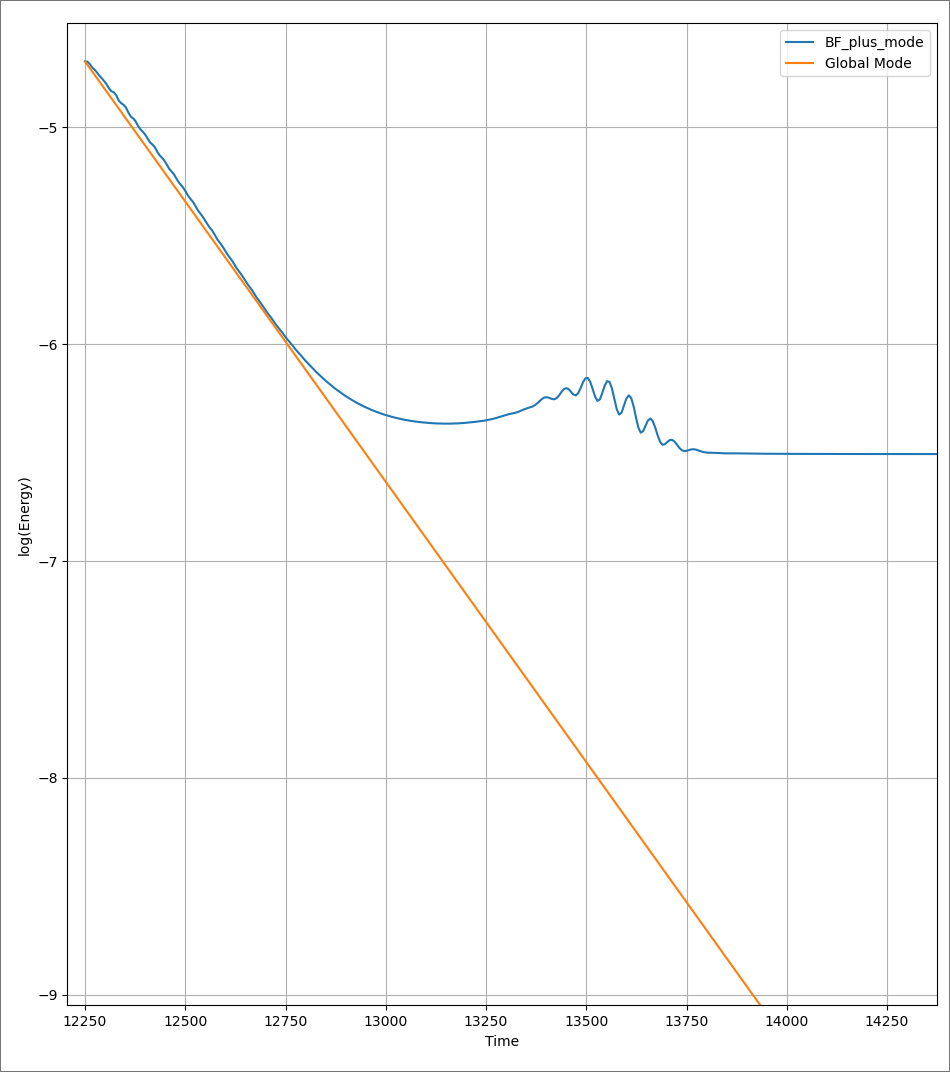
\includegraphics[width=0.7\linewidth]{Images/plot.png}

			v-component L2 norm comparison
		}
	\end{column}
	\end{columns}

        
\end{frame}
\begin{frame}
	\frametitle{weird wiggles}

	{
	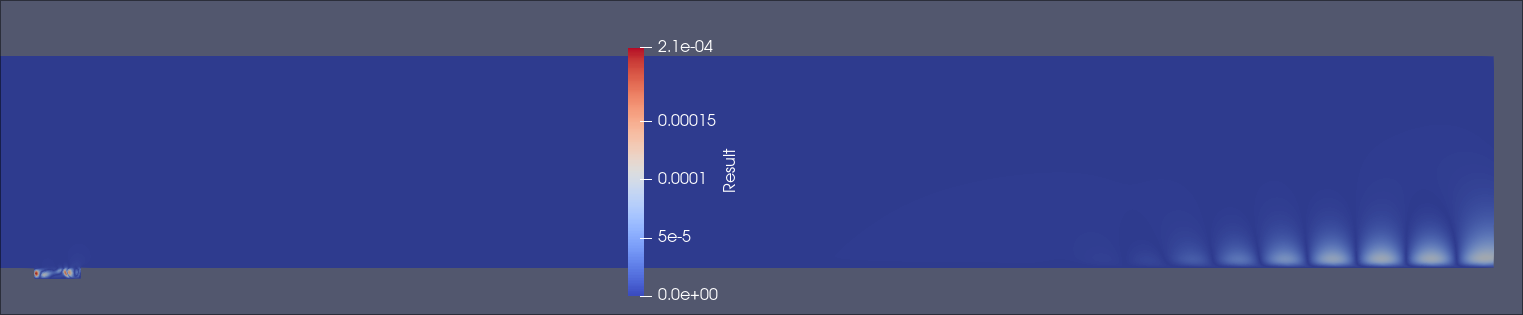
\includegraphics[width=\linewidth]{Images/weirdTS.png}
	}
\end{frame}
\begin{frame}
	\frametitle{3rd test}
	\begin{itemize}
		\item Compute growth rate of global modes for a case with wider gap. 
		\item I chose $w = 18\delta^*$ but I \textbf{forgot} to disable the SVV.
		\item Still running the EV solver, but it looks again negative growth rate.
		\item Could it be that SVV is damping too much the modes?
	\end{itemize}
	
\end{frame}

\end{document}
